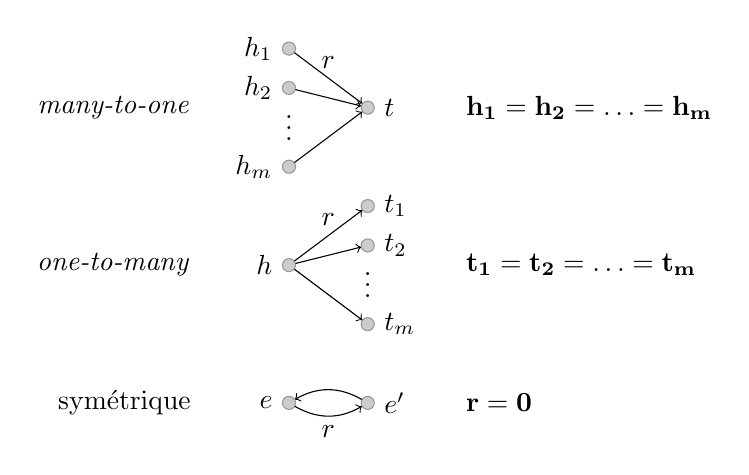
\begin{tikzpicture}
        [
            neuron/.style={draw=black!40, fill=black!20, circle, scale=0.5},
            rel/.style={draw=black}
        ]
    \def\ox{0.5}
    \def\oy{0.5}
	\node [neuron, label={180:$h_1$}] (0) at (0*\ox, 3*\oy) {};
	\node [neuron, label={180:$h_2$}] (1) at (0*\ox, 2*\oy) {};
	\node at (0*\ox, 1.2*\oy) {$\vdots$};
	\node [neuron, label={180:$h_m$}] (3) at (0*\ox, 0*\oy) {};
	\node [neuron, label={0:$t$}] (4) at (2*\ox, 1.5*\oy) {};
	\node [neuron, label={180:$h$}] (10) at (0*\ox, -2.5*\oy) {};
	\node [neuron, label={0:$t_1$}] (5) at (2*\ox, -1*\oy) {};
	\node [neuron, label={0:$t_2$}] (6) at (2*\ox, -2*\oy) {};
	\node at (2*\ox, -2.8*\oy) {$\vdots$};
	\node [neuron, label={0:$t_m$}] (7) at (2*\ox, -4*\oy) {};
	\node [neuron, label={180:$e$}] (8) at (0*\ox, -6*\oy) {};
	\node [neuron, label={0:$e'$}] (9) at (2*\ox, -6*\oy) {};
	\node [label={180:{\textit{many-to-one}}}] (11) at (-2*\ox, 1.5*\oy) {};
	\node [label={180:{\textit{one-to-many}}}] (12) at (-2*\ox, -2.5*\oy) {};
	\node [label={180:{symétrique}}] (13) at (-2*\ox, -6*\oy) {};
	\node[label={0:$\implies \mathbf{h_1} = \mathbf{h_2} = \ldots = \mathbf{h_m}$}] (14) at  (4*\ox, 1.5*\oy) {};
	\node[label={0:$\implies \mathbf{t_1} = \mathbf{t_2} = \ldots = \mathbf{t_m}$}] (15) at  (4*\ox, -2.5*\oy) {};
	\node[label= {0:$\implies \mathbf{r} = \mathbf{0}$}] (16) at  (4*\ox, -6*\oy) {};
		
		\draw [style=rel, ->] (0) to node[above]{$r$} (4);
		\draw [style=rel, ->] (1) to (4);
		\draw [style=rel, ->] (3) to (4);
		\draw [style=rel, bend right, ->] (8) to node[below]{$r$} (9);
		\draw [style=rel, ->] (10) to node[above]{$r$} (5);
		\draw [style=rel, ->] (10) to (6);
		\draw [style=rel, ->] (10) to (7);
		\draw [style=rel, bend left, <-] (8) to (9);
        \end{tikzpicture}